\documentclass[aspectratio=169]{beamer}
\usepackage[english]{babel}
\usepackage[T1]{fontenc}
\usepackage[utf8]{inputenc}
\usepackage{cite}
\usepackage{tikz}
%\usetikzlibrary{shapes,arrows,fit,calc,positioning,automata}
\usepackage{eurosym}
\usepackage{caption}
\captionsetup[figure]{labelformat=empty}

%\setbeamertemplate{navigation symbols}{}
%\usepackage{beamerthemeshadow}


\title{Development and test of FPGA firmware for the readout of the ABACUS chip for beam monitoring applications in hadron therapy}
\author[Stefan Zugravel]{Candidate: \\ Stefan Cristi Zugravel \\ --------------------------------- \\ Supervisor: \\ Prof. Luca Pacher\\ ---------------------------------  \\ Co-Supervisor: \\ Prof. Vincenzo Monaco}
\date{\today}
\institute[UniTo]{University of Turin}
\logo{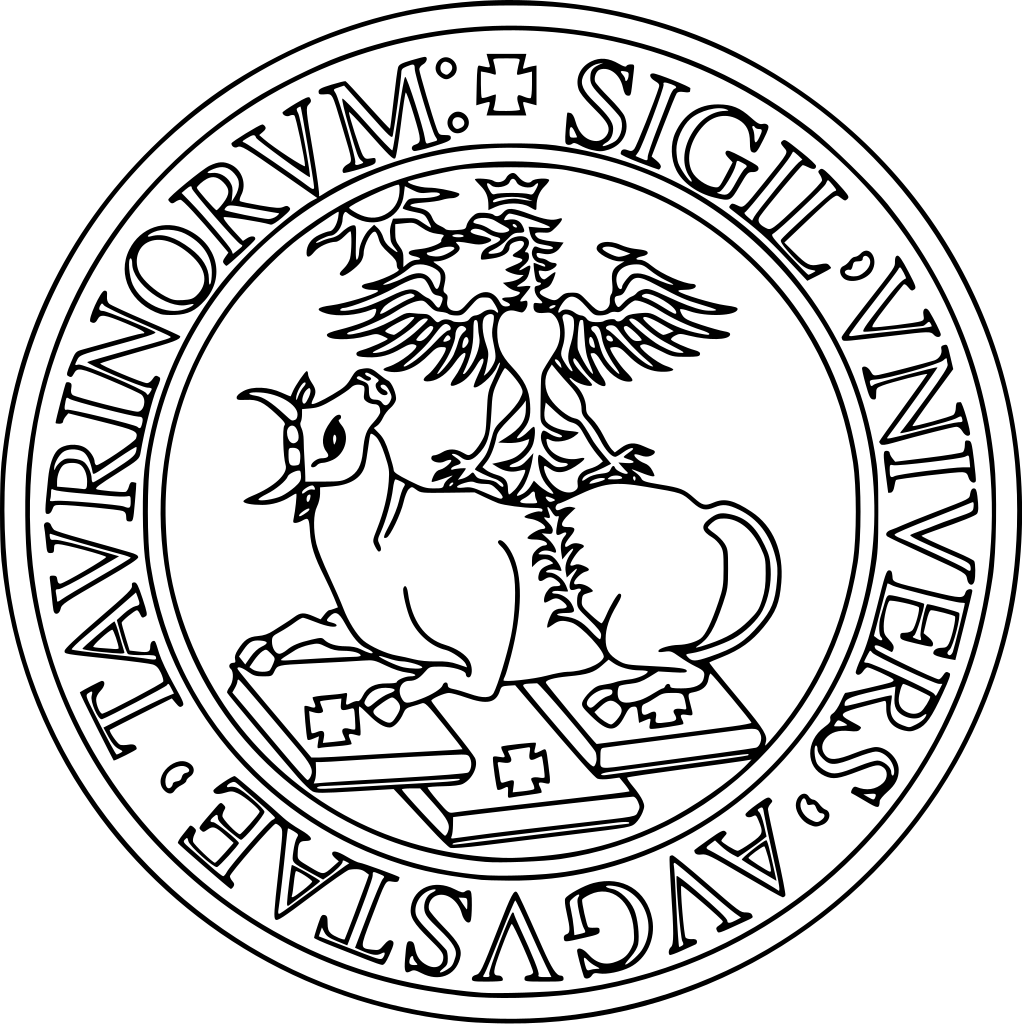
\includegraphics[width=10mm]{IMG/Unito}}
%\usetheme{Antibes}
\usetheme{Madrid}
%\setbeamercovered{dynamic}
\setbeamertemplate{footline}[frame number]
%\beamertemplatenavigationsymbolsempty
\setbeamertemplate{navigation symbols}{}
\begin{document}
	
	\begin{frame}		
		\maketitle
	\end{frame}

	\begin{frame}
	\frametitle{Table of contents}
		\begin{columns}
			\column{0.3 \textwidth}
				\begin{center}
					\tableofcontents
				\end{center}
			\column{0.7 \textwidth}
				\begin{center}
					
\includegraphics[width=0.95 \textwidth]{IMG/Move_IT_logo.PNG}
				\end{center}
		\end{columns}	
	\end{frame}

%%%%%%%%%%%%%%%%%%%%%%%%%%%%%%%%%%%%%%%%%%%%%%%%%%%%%%%%%%%%%%%%%%%%%%%%%%%%%%%%%%%%%%%%
	\section{Hadron therapy}
	
	\begin{frame}
	\frametitle{Hadron therapy}
	\begin{columns}
		\column{0.50 \textwidth}
		\begin{center}
			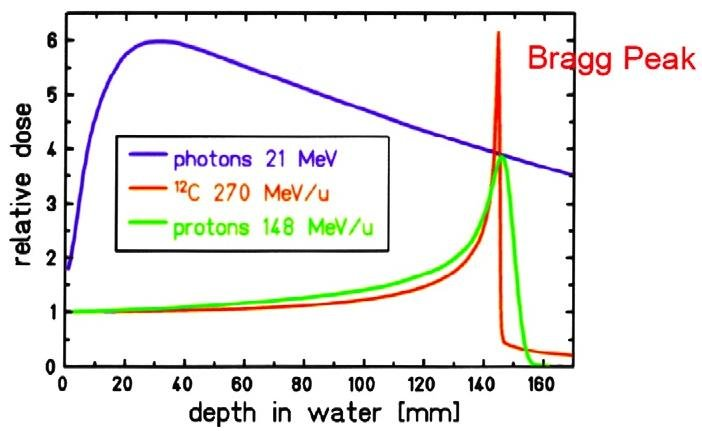
\includegraphics[width=0.75 \textwidth]{IMG/Bragg_Peak.PNG}
			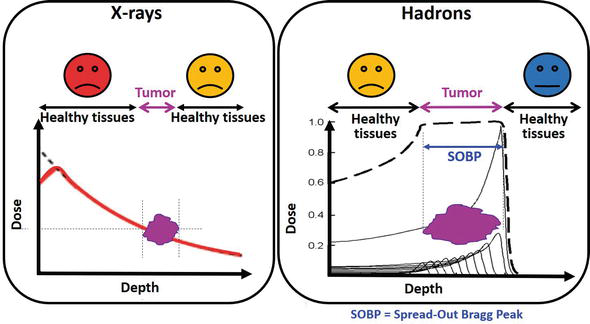
\includegraphics[width=0.65 \textwidth]{IMG/Bragg_Peak2.PNG}
		\end{center}
		\column{0.50 \textwidth}
		\begin{center}
			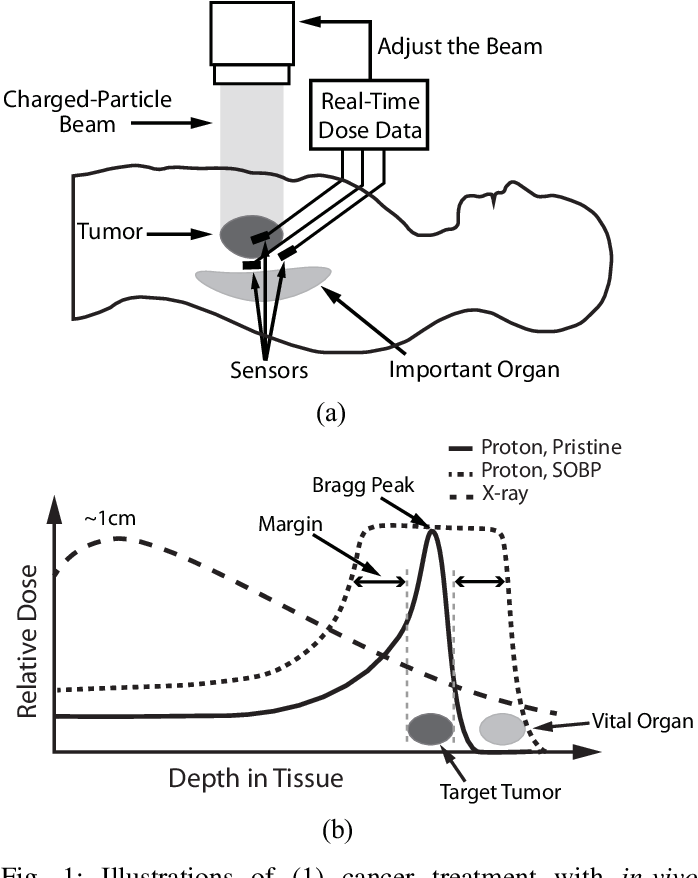
\includegraphics[width=0.55 \textwidth]{IMG/HadroTherapy.PNG}
			\newline
			{\color{red} aggiungere informazioni sull'adrotepia}
		\end{center}
	\end{columns}
	
	\end{frame}

%%%%%%%%%%%%%%%%%%%%%%%%%%%%%%%%%%%%%%%%%%%%%%%%%%%%%%%%%%%%%%%%%%%%%%%%%%%%%%%%%%%%%%%%
	\section{LGAD sensors}
	
	\begin{frame}
	\frametitle{LGAD sensors}
	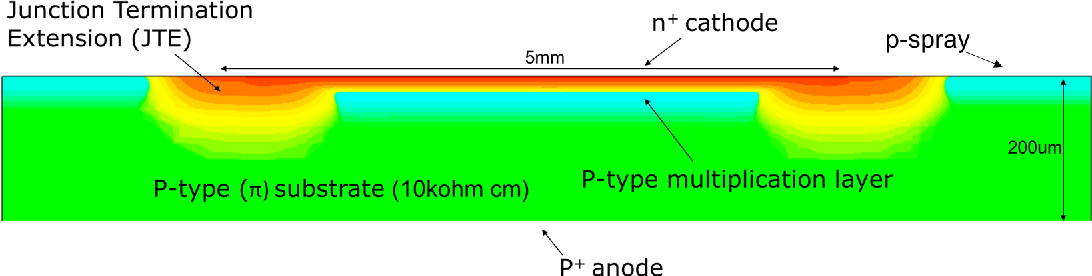
\includegraphics[width=0.95 \textwidth]{IMG/LGAD_image.PNG}
	\newline
	{\color{red} aggiungere informazioni su LGAD}
	\end{frame}

%%%%%%%%%%%%%%%%%%%%%%%%%%%%%%%%%%%%%%%%%%%%%%%%%%%%%%%%%%%%%%%%%%%%%%%%%%%%%%%%%%%%%%%%
	\section{ABACUS2 Asic}
	
	\begin{frame}
	\frametitle{ABACUS2}
	{\color{red} aggiungere informazioni su ABACUS2}
	\end{frame}

	\begin{frame}
	\frametitle{ABACUS2}
	{\color{red} seconda slide in cui parlerò di abacus 2}
	\end{frame}

%%%%%%%%%%%%%%%%%%%%%%%%%%%%%%%%%%%%%%%%%%%%%%%%%%%%%%%%%%%%%%%%%%%%%%%%%%%%%%%%%%%%%%%%
	\section{FPGA}
	
	\begin{frame}
	\frametitle{FPGA board }
	\begin{center}
		Kintex7 kc705 board
		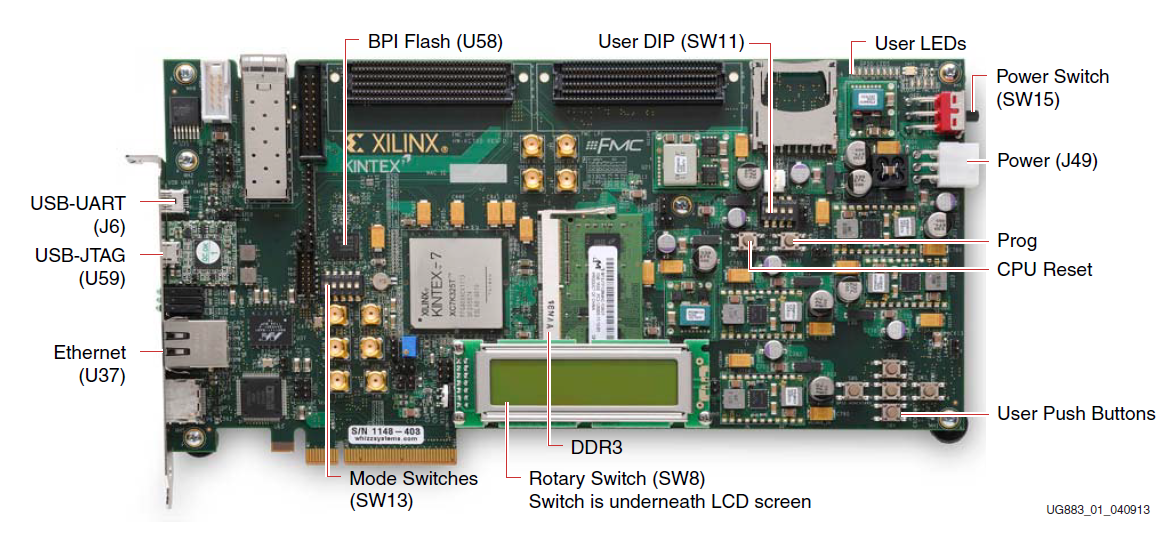
\includegraphics[width=0.85 \textwidth]{IMG/Kintex7_board.PNG}
	\end{center}
	\end{frame}

	\begin{frame}
	\frametitle{Test bench}
	\begin{center}
		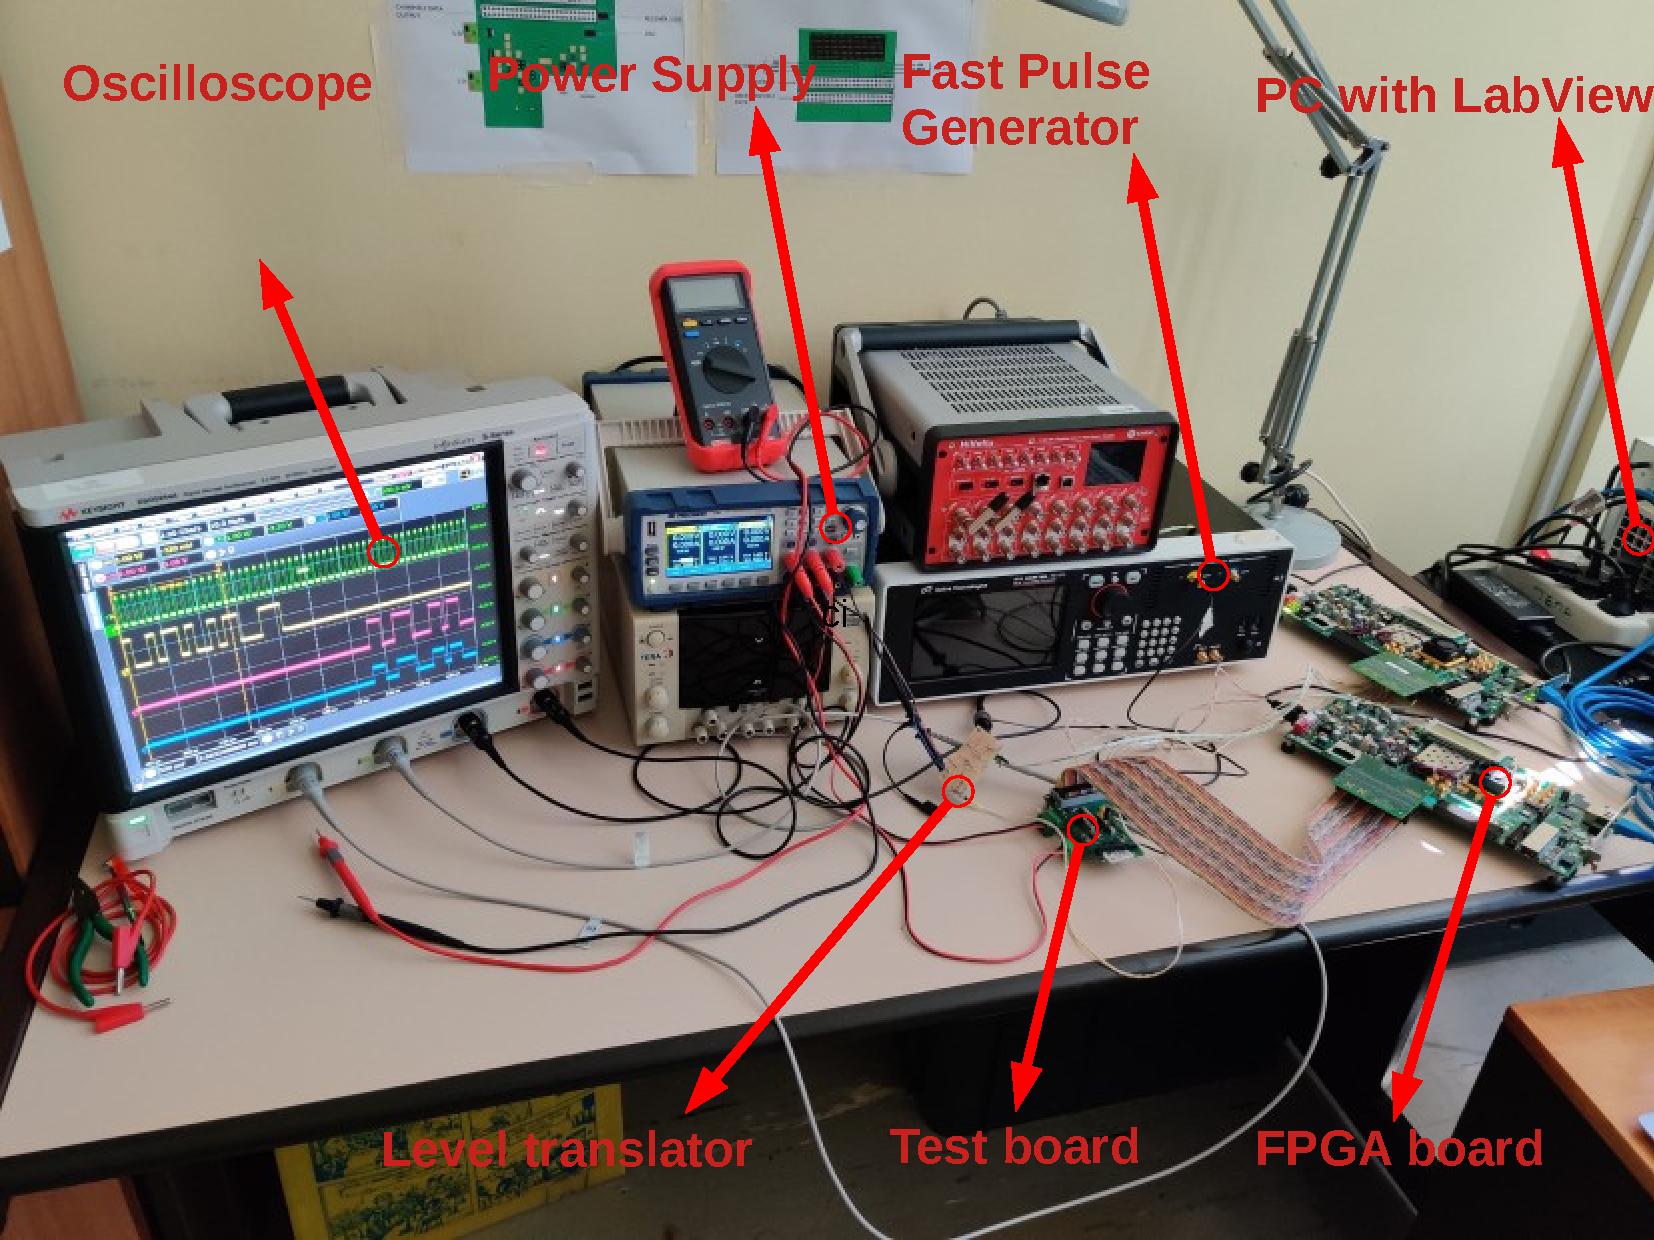
\includegraphics[width=0.65 \textwidth]{IMG/TestBench.pdf}
	\end{center}
	\end{frame}

	\begin{frame}
	\frametitle{Test board}
	\begin{center}
		Test board with ABACUS2 ASIC
		%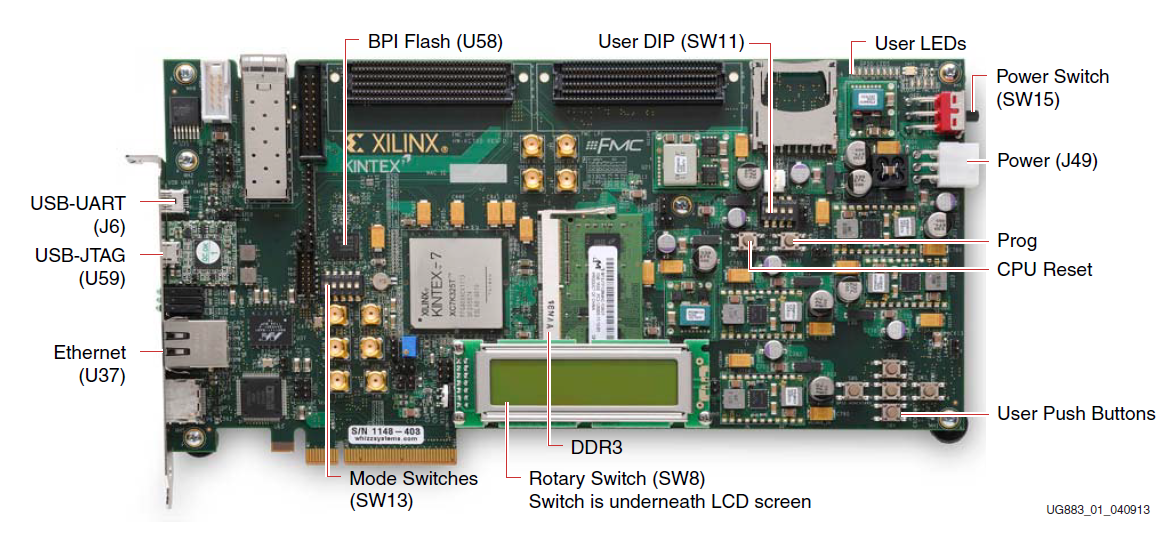
\includegraphics[width=0.85 \textwidth]{IMG/Kintex7_board.PNG}
	\end{center}
	\end{frame}

	
%%%%%%%%%%%%%%%%%%%%%%%%%%%%%%%%%%%%%%%%%%%%%%%%%%%%%%%%%%%%%%%%%%%%%%%%%%%%%%%%%%%%%%%%
	\section{Firmware}
	
	\begin{frame}[fragile]
	\frametitle{Debug Tool}
	\begin{center}
		{\small \color{blue} Step1: Signal names and identification.}
	\end{center}
	{\tiny
		\begin{verbatim}
			pin68				: out std_logic;--H4  FMC_HPC_CLK0_M2C_P    LVDS D27         -P3 + v
			pin69				: out std_logic;--H5  FMC_HPC_CLK0_M2C_N    LVDS C27         -P4 - v 
		\end{verbatim} }
	\begin{center}
		{\small \color{blue} Step2: Differential Signalling output buffer.}
	\end{center}
	{\tiny
		\begin{verbatim}
		attribute IOSTANDARD of pin68_OBUFDS : label is "LVDS_25";	
		pin68_OBUFDS : unisim.vcomponents.OBUFDS
		port map (
		I		=> pin68_int,
		O		=> pin68,
		OB		=> pin69);		
		\end{verbatim} }
	\begin{center}
		{\small \color{blue} Step3: Constraints settings.}
	\end{center}
	{\tiny
		\begin{verbatim}
		# FMC_HPC_CLK0_M2C_P
		# FMC_HPC_CLK0_M2C_N
		set_property -dict { PACKAGE_PIN D27	IOSTANDARD LVDS_25 DIFF_TERM TRUE }	[get_ports pin68]
		set_property -dict { PACKAGE_PIN C27	IOSTANDARD LVDS_25 DIFF_TERM TRUE }	[get_ports pin69]
		\end{verbatim} }
	\end{frame}

	\begin{frame}
	\frametitle{Writing Baseline DACs $\rightarrow$ code}
	
	\end{frame}

	\begin{frame}
	\frametitle{Writing Baseline DACs $\rightarrow$ clock stats}
	\begin{center}
		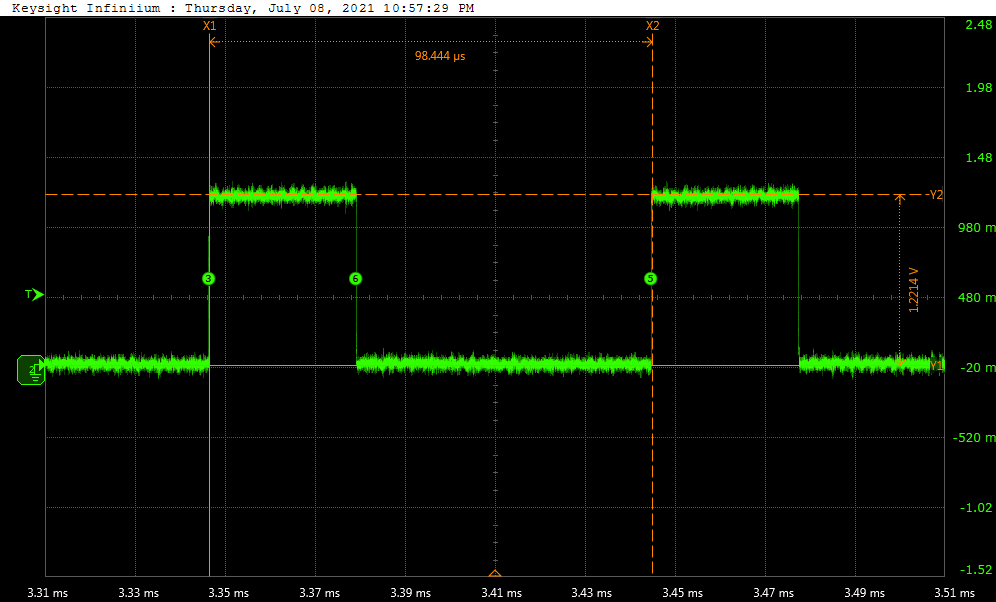
\includegraphics[width=0.65 \textwidth]{IMG/probe/09-08-2021_clock-specks.png}
	\end{center}
	\end{frame}

	\begin{frame}
	\frametitle{Writing Baseline DACs $\rightarrow$ clock stats}
	\begin{center}
		\begin{figure}
			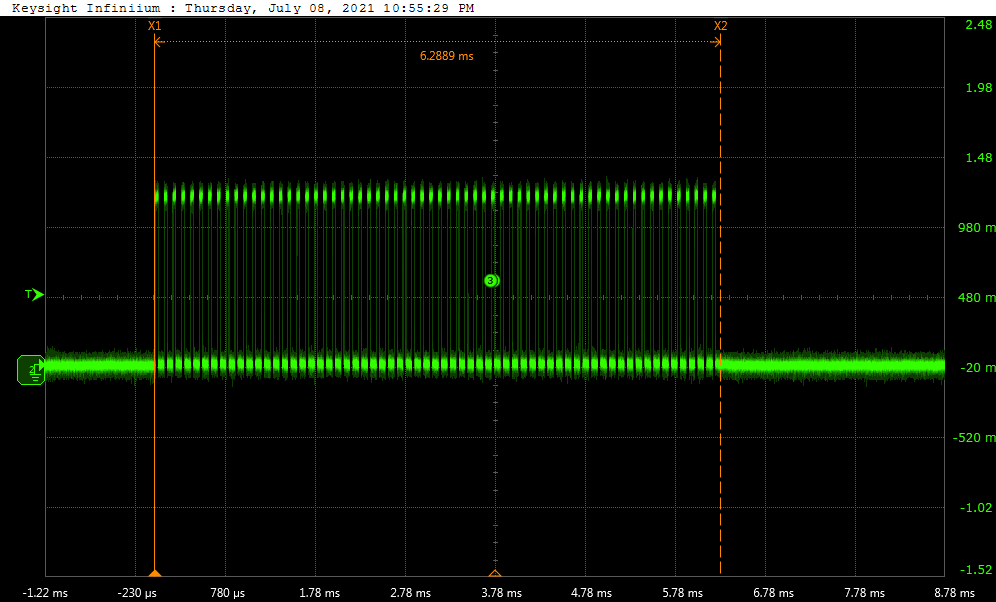
\includegraphics[width=0.65 \textwidth]{IMG/probe/09-08-2021_packet-time.png}
			\caption{{\small packet time}}
		\end{figure}
		
		
	\end{center}
	\end{frame}

	\begin{frame}
	\frametitle{Writing Baseline DACs $\rightarrow$ data}
	\begin{columns}
		\column{0.50 \textwidth}
		\begin{center}
			\begin{figure}
				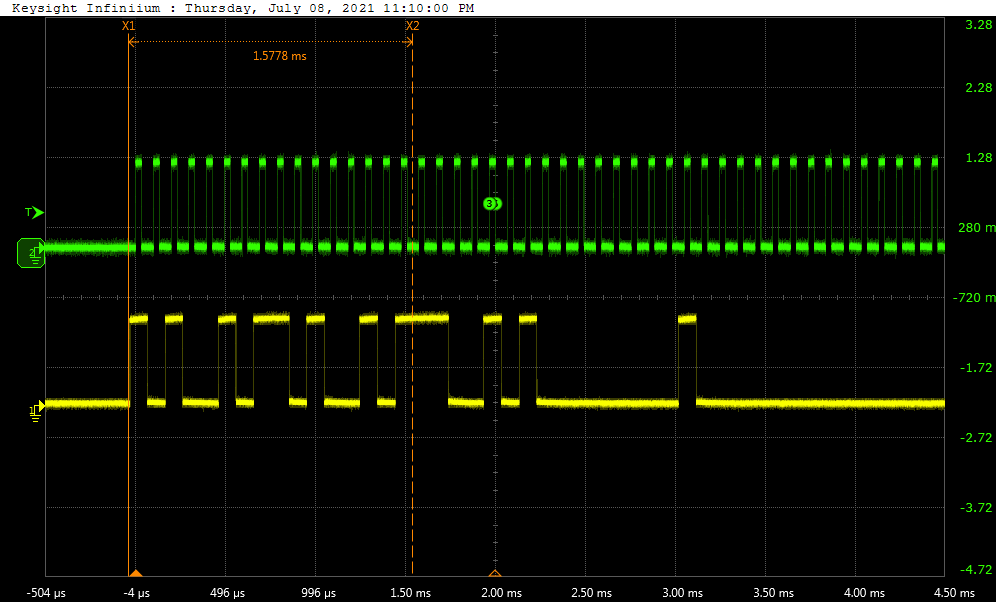
\includegraphics[width=0.55 \textwidth]{IMG/probe/09-08-2021_ch05-write01-baselinedac1.png}
				\caption{\centering{\tiny 11-001010-00000001 ch05-write01-baselinedac1}}
			\end{figure}
			\begin{figure}
				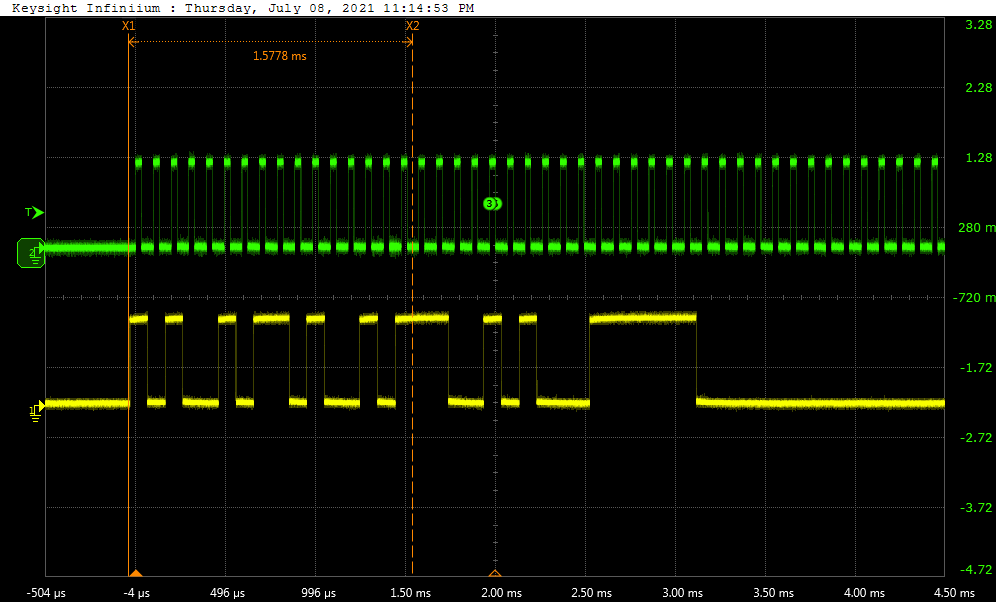
\includegraphics[width=0.55 \textwidth]{IMG/probe/09-08-2021_ch05-write63-baselinedac1.png}
				\caption{\centering{\tiny 11-001010-00111111 ch05-write63-baselinedac1}}
			\end{figure}		
		\end{center}
		\column{0.50 \textwidth}
		
		\begin{center}
			\begin{figure}
				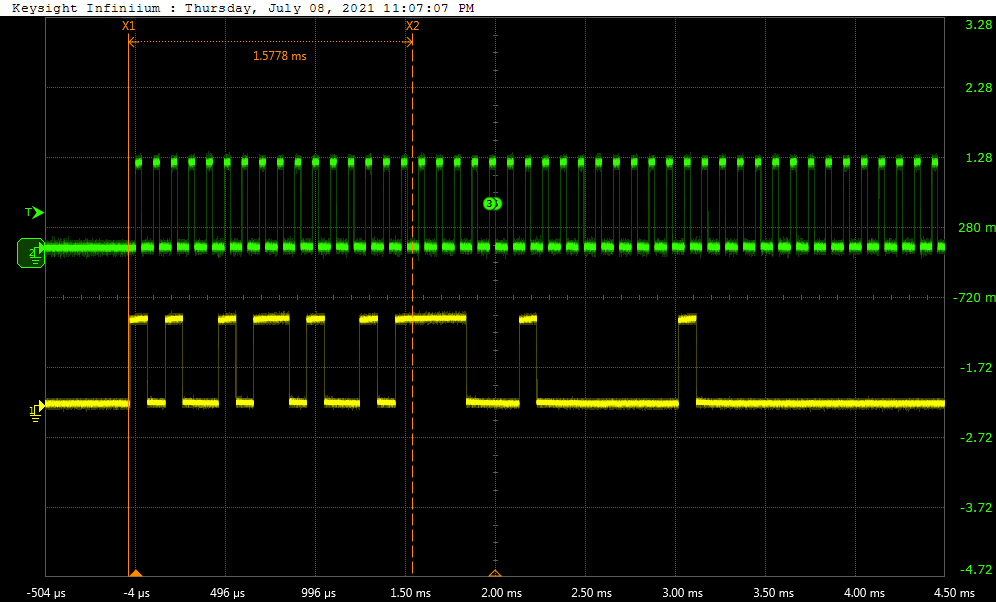
\includegraphics[width=0.55 \textwidth]{IMG/probe/09-08-2021_ch17-write01-baselinedac1.png}
				\caption{\centering{\tiny 11-100010-00000001 ch17-write01-baselinedac1}}
			\end{figure}
			\begin{figure}
				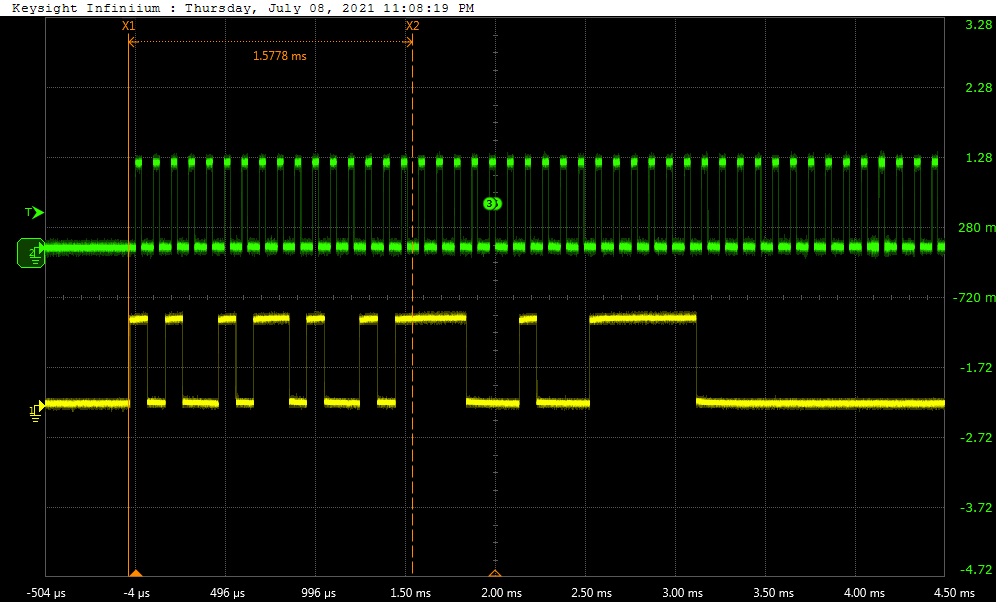
\includegraphics[width=0.55 \textwidth]{IMG/probe/09-08-2021_ch17-write63-baselinedac1.png}
				\caption{\centering{\tiny 11-100010-00111111 ch17-write63-baselinedac1}}
			\end{figure}	
		\end{center}
	\end{columns}
	\end{frame}

	\begin{frame}
	\frametitle{Reading Baseline DACs $\rightarrow$ code}

	\end{frame}

	\begin{frame}
	\frametitle{Level translator}
	
	\end{frame}

	\begin{frame}
	\frametitle{Reading Baseline DACs $\rightarrow$ data}
	\begin{columns}
		\column{0.50 \textwidth}
		\begin{center}
			\begin{figure}
				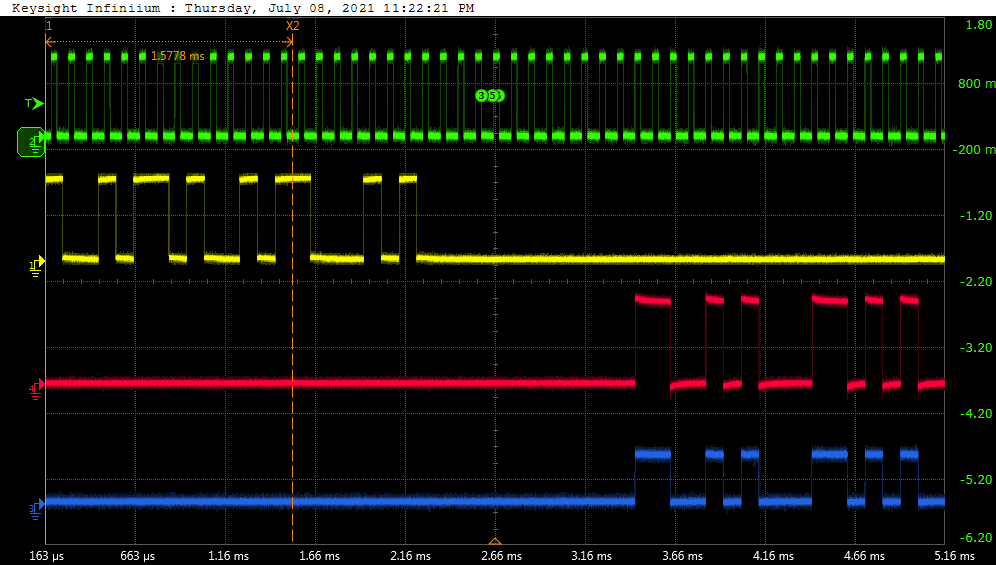
\includegraphics[width=0.55 \textwidth]{IMG/probe/09-08-2021_ch05-read53-baselinedac1.png}
				\caption{\centering{\tiny 11-001010-00000001 ch05-write01-baselinedac1}}
			\end{figure}
			\begin{figure}
				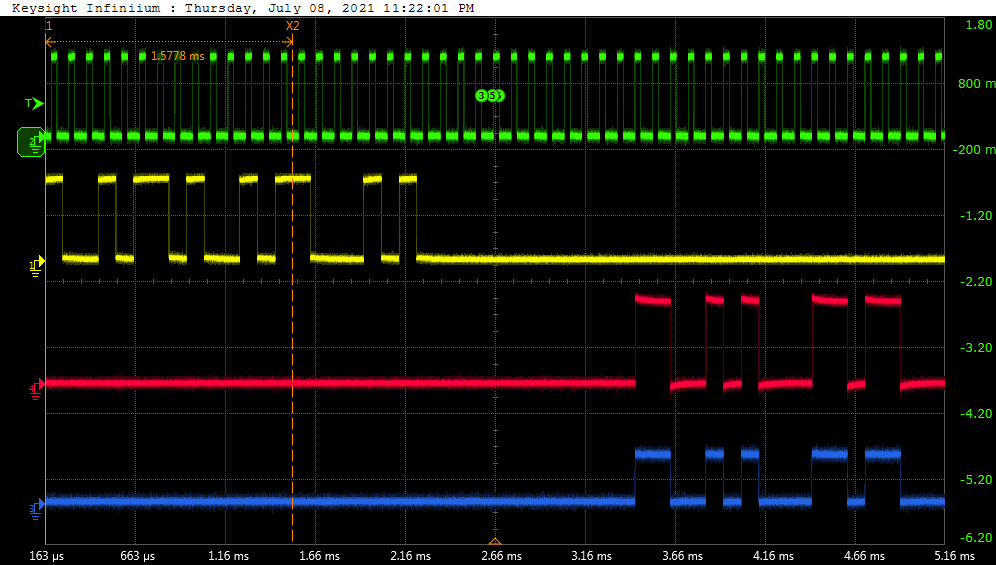
\includegraphics[width=0.55 \textwidth]{IMG/probe/09-08-2021_ch05-read54-baselinedac1.png}
				\caption{\centering{\tiny 11-001010-00111111 ch05-write63-baselinedac1}}
			\end{figure}		
		\end{center}
		\column{0.50 \textwidth}
		
		\begin{center}
			\begin{figure}
				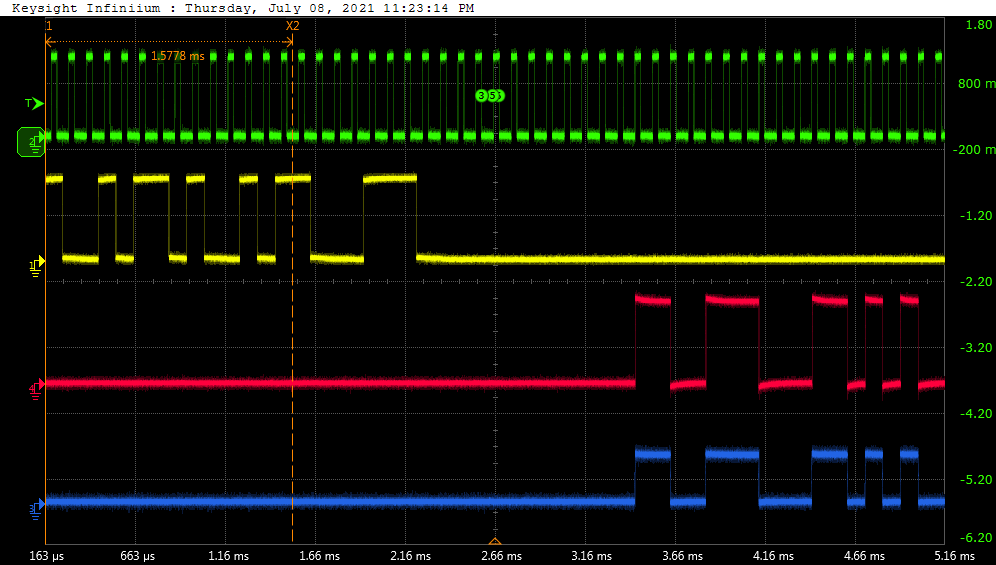
\includegraphics[width=0.55 \textwidth]{IMG/probe/09-08-2021_ch07-read53-baselinedac1.png}
				\caption{\centering{\tiny 11-100010-00000001 ch17-write01-baselinedac1}}
			\end{figure}
			\begin{figure}
				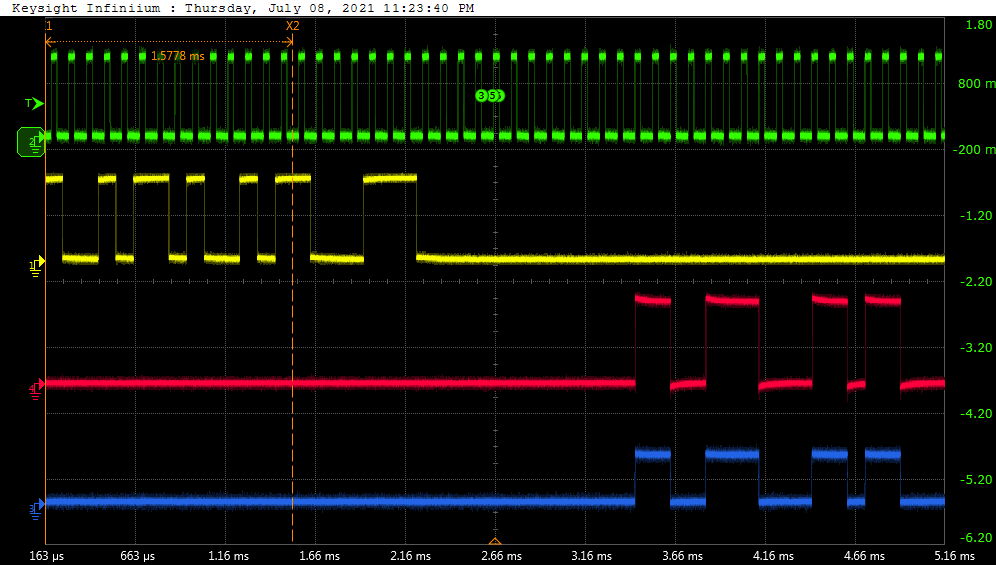
\includegraphics[width=0.55 \textwidth]{IMG/probe/09-08-2021_ch07-read54-baselinedac1.png}
				\caption{\centering{\tiny 11-100010-00111111 ch17-write63-baselinedac1}}
			\end{figure}	
		\end{center}
	\end{columns}
	\end{frame}

%%%%%%%%%%%%%%%%%%%%%%%%%%%%%%%%%%%%%%%%%%%%%%%%%%%%%%%%%%%%%%%%%%%%%%%%%%%%%%%%%%%%%%%%
	\section{Constraints}
	
	\begin{frame}[fragile]
	\frametitle{Constraints}
	{\tiny 
		\begin{verbatim}
			##Single-ended signal for baseline dac1#######################################
			# FMC_HPC_LA01_CC_P
			set_property -dict { PACKAGE_PIN D26	IOSTANDARD LVCMOS25 DIFF_TERM TRUE}	[get_ports baseline_dac1_sck]
			# FMC_HPC_LA01_CC_N
			set_property -dict { PACKAGE_PIN C26	IOSTANDARD LVCMOS25 DIFF_TERM TRUE}	[get_ports gnd_10]
			#
			# FMC_HPC_LA06_P
			set_property -dict { PACKAGE_PIN H30	IOSTANDARD LVCMOS25 DIFF_TERM TRUE}	[get_ports baseline_dac1_mosi]
			# FMC_HPC_LA06_N
			set_property -dict { PACKAGE_PIN G30	IOSTANDARD LVCMOS25 DIFF_TERM TRUE}	[get_ports gnd_11]
			#
			# FMC_HPC_LA05_P
			set_property -dict { PACKAGE_PIN G29	IOSTANDARD LVCMOS25 DIFF_TERM TRUE}	[get_ports baseline_dac1_miso]
			# FMC_HPC_LA05_N
			set_property -dict { PACKAGE_PIN F30	IOSTANDARD LVCMOS25 DIFF_TERM TRUE}	[get_ports gnd_12]
				
		\end{verbatim} 
	}

		\color{red} Da aggiungere spiegazione
	\end{frame}

%%%%%%%%%%%%%%%%%%%%%%%%%%%%%%%%%%%%%%%%%%%%%%%%%%%%%%%%%%%%%%%%%%%%%%%%%%%%%%%%%%%%%%%%
	\section{Results}
	
	\begin{frame}
	\frametitle{7 }
	
		\begin{center}
			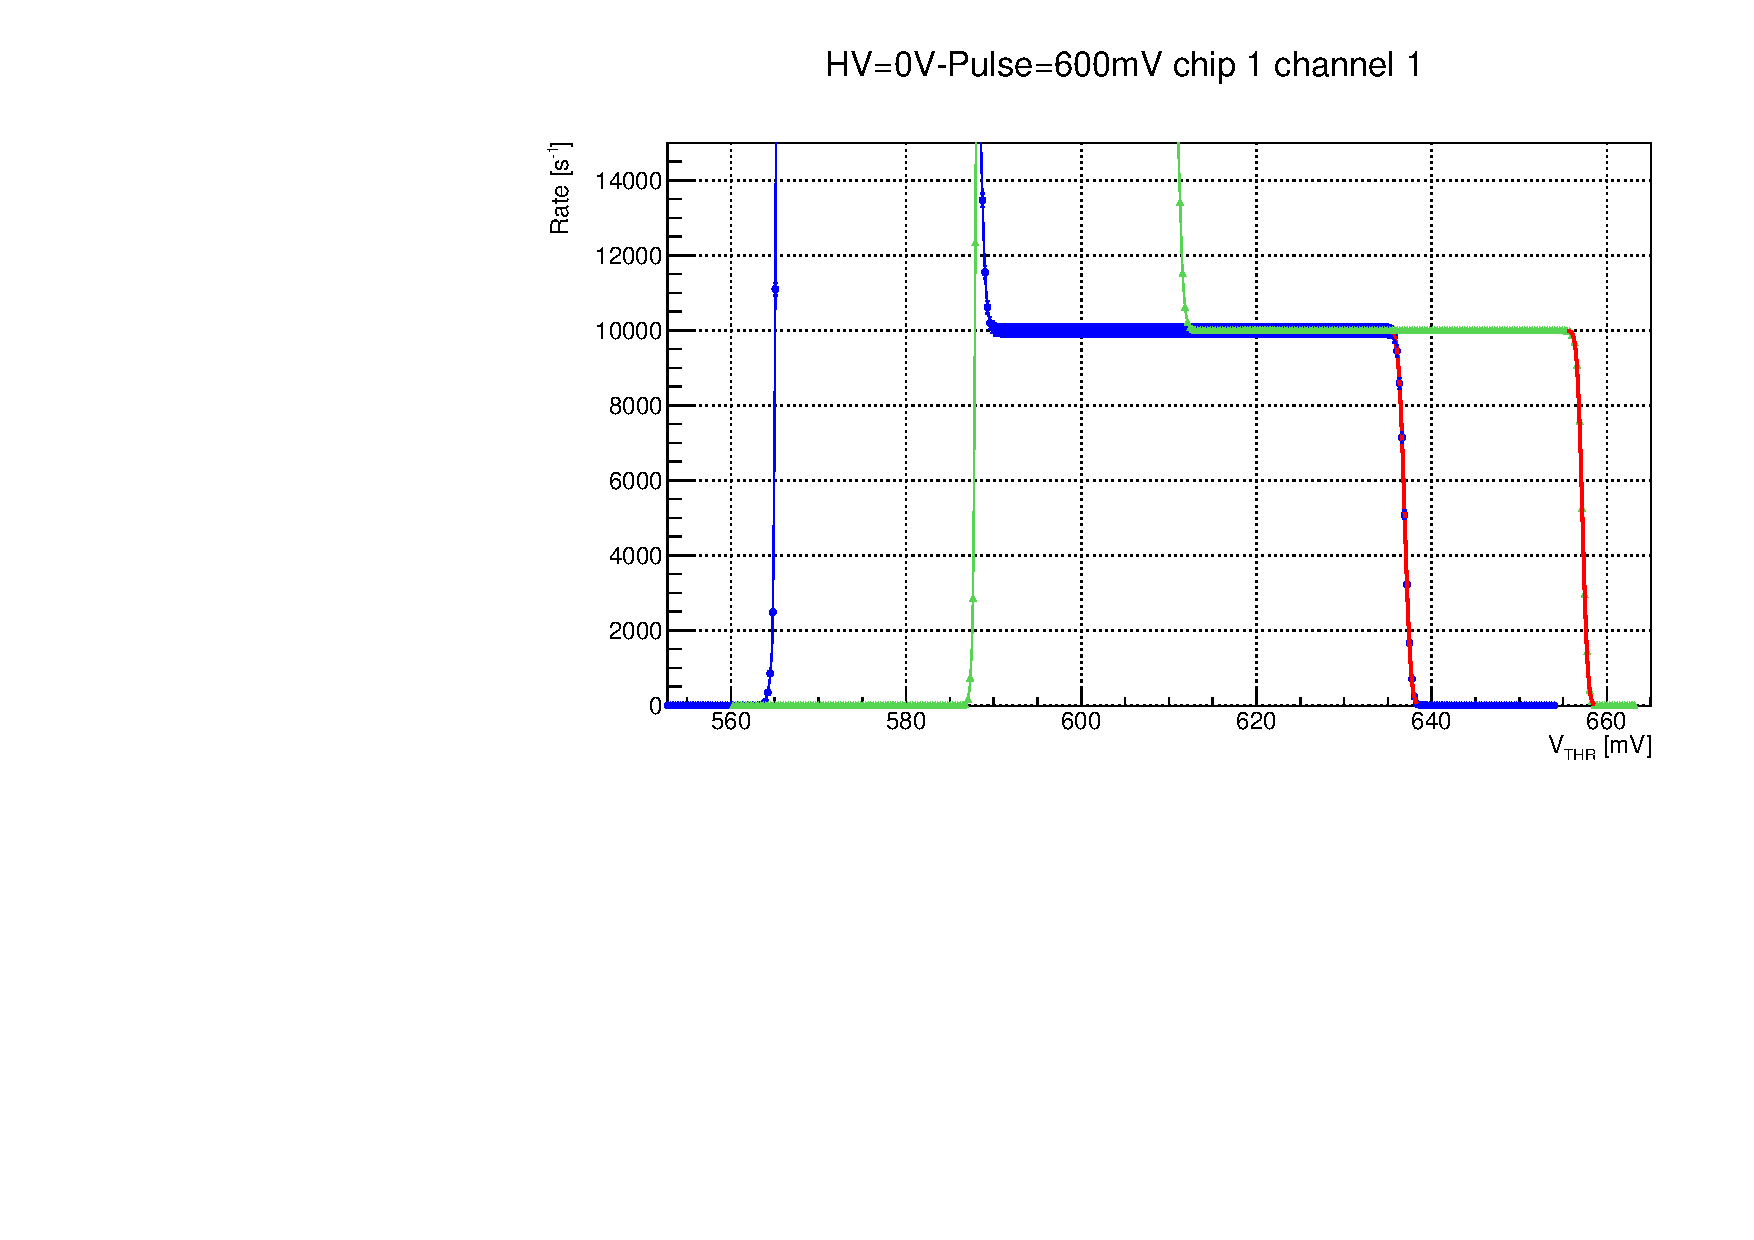
\includegraphics[width=0.75 \textwidth]{IMG/ThScan_ch0.pdf}
		\end{center}
	
	\color{red}  qua spiego il grafico e cosa rappresenta
	
	\end{frame}

	\begin{frame}
	\frametitle{8 }
	
	\begin{center}
		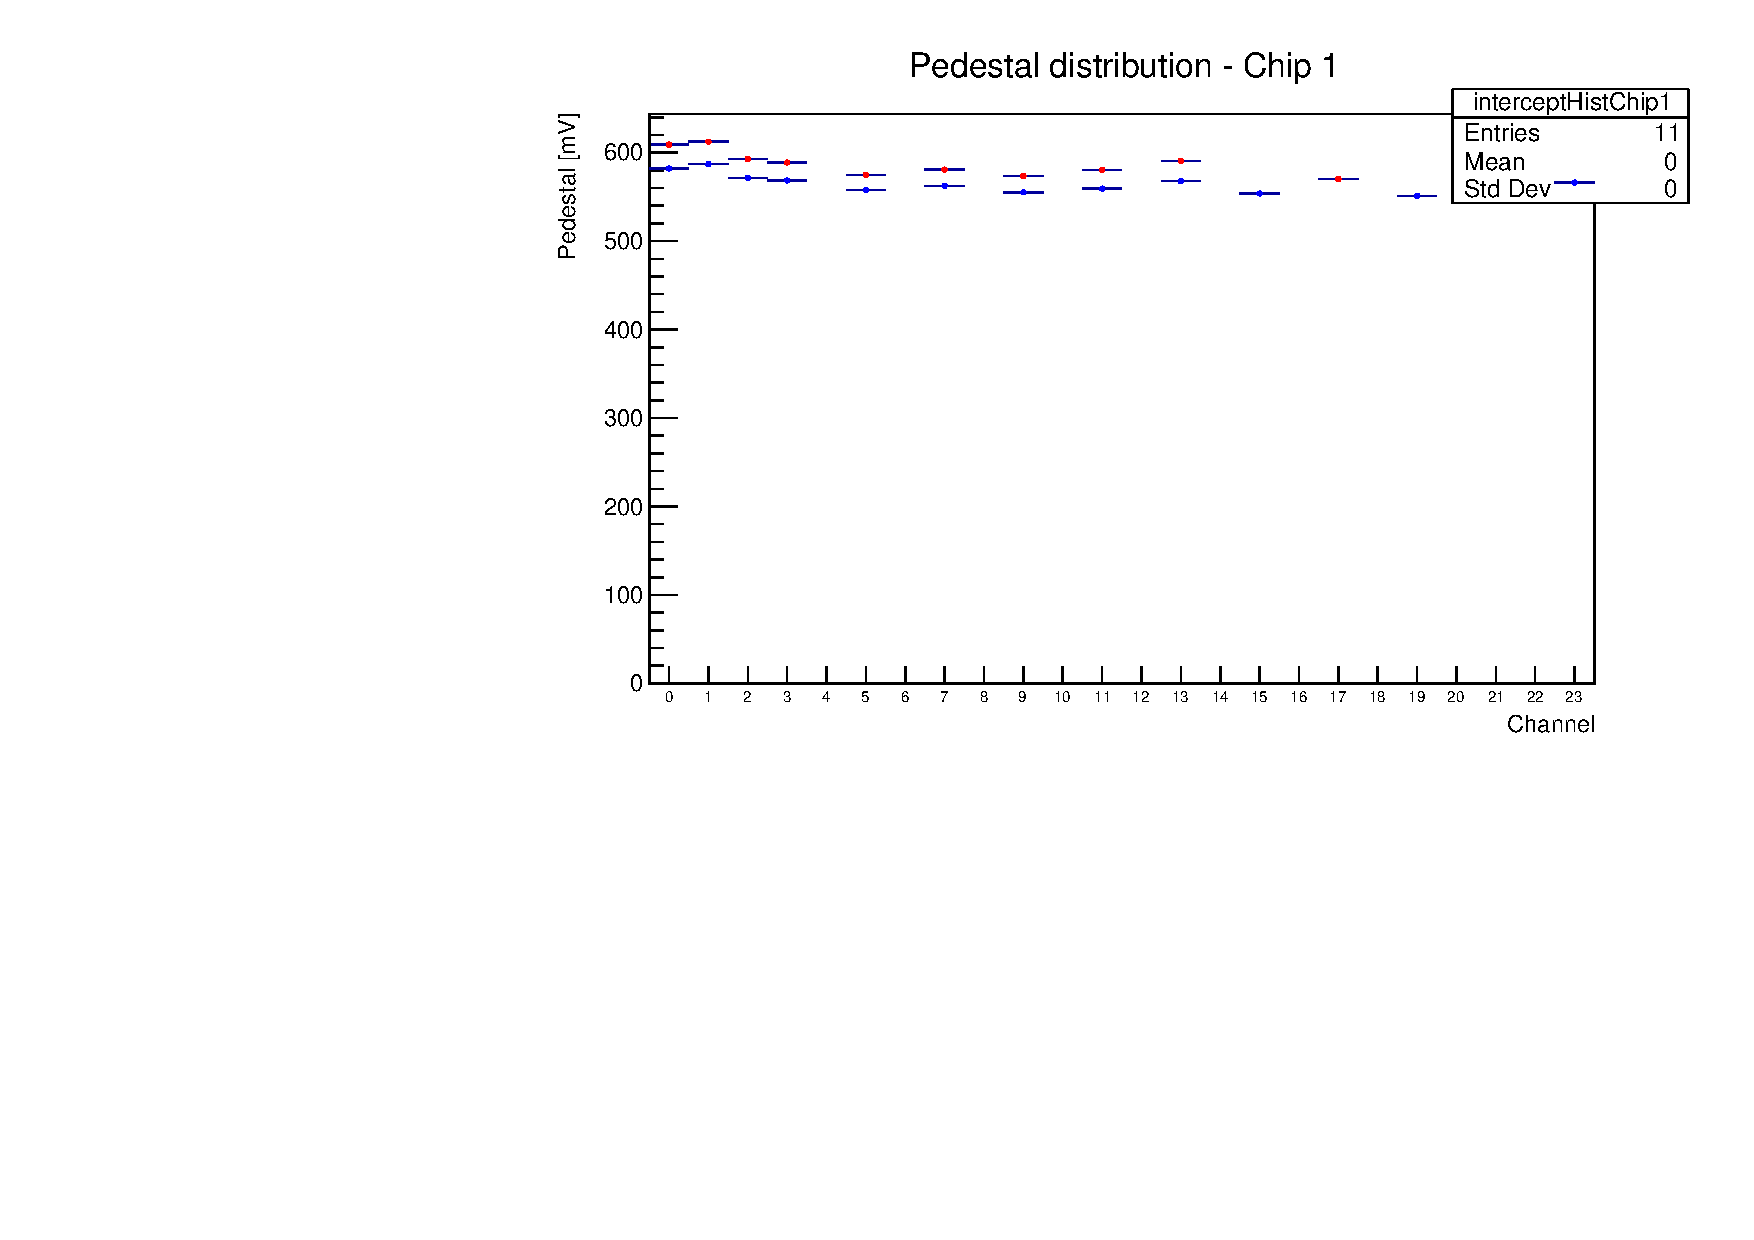
\includegraphics[width=0.75 \textwidth]{IMG/TB1-DAC0-DAC63.pdf}
	\end{center}
	
	\color{red}  qua spiego il grafico e cosa rappresenta
	
	\end{frame}

%%%%%%%%%%%%%%%%%%%%%%%%%%%%%%%%%%%%%%%%%%%%%%%%%%%%%%%%%%%%%%%%%%%%%%%%%%%%%%%%%%%%%%%%
	\section{Conclusions}
	
	\begin{frame}
	\frametitle{Conclusions }
	\begin{center}
		\textbf{Future additions to the FPGA firmware}
	\end{center}
		\begin{itemize}
			\item timestamp
			\item latched counters
			
		\end{itemize}
		\begin{center}
			Thanks for the attention
		\end{center}
		
	\end{frame}

	\begin{frame}
	\frametitle{Bibliography}
	{\small
	\begin{thebibliography}{00}
		\bibitem{1}www.researchgate.net/figure/Dose-depth-curve-for-monoenergetic-photons-protons-and-carbon-ions-courtesy-of-GSI$\textunderscore$fig1$\textunderscore$283521369
		\newline
		\bibitem{2}www.intechopen.com/books/novel-prospects-in-oxidative-and-nitrosative-stress/oxidative-stress-in-hadrontherapy
		\newline
		\bibitem{3}www.semanticscholar.org/paper/A-Millimeter-Scale-Single-Charged-Particle-for-Lee-Scholey/ae955a07a42e9c124a8473357cd485b0b9928090
		\newline
		\bibitem{4}www.semanticscholar.org/paper/Low-Gain-Avalanche-Detectors-(LGAD)-for-particle-Moffat-Bates/0477d7bc2c9a3b26ad776874598f56d7d5b54c45
	\end{thebibliography} }
	\end{frame}

%%%%%%%%%%%%%%%%%%%%%%%%%%%%%%%%%%%%%%%%%%%%%%%%%%%%%%%%%%%%%%%%%%%%%%%%%%%%%%%%%%%%%%%%
	\section{Auxiliary images}
	
	\begin{frame}
	\frametitle{Additional Graphs}
	
	\end{frame}

\end{document}